\chapter{Classification}

Per la costruzione dei classificatori abbiamo adottato lo stesso dataset
usato per DBSCAN, ovvero costituito dai soli attributi relativi ai
\texttt{payment status}. Questo ci ha permesso di ottenere le migliori
performance.

Si \`e operata una grid search con i seguenti range di valori degli attributi:
\begin{itemize}
	\item \texttt{min\_samples\_split} $\in [2, 5, 10, 20, 100, 150, 250]$
	\item \texttt{min\_samples\_leaf} $\in [1, 5, 10, 20, 100]$
	\item \texttt{criterion} $\in [gini, entropy]$
	\item \texttt{max\_features} $\in [None, log2, sqrt]$
	\item \texttt{min\_impurity\_decrease} $\in [1^{-6}, 1^{-7}, 1^{-8}, 0]$
	\item \texttt{max\_depth} $\in [None, 2, 4, 7, 10]$
\end{itemize}

Il risultato \`e stata l'individuazione di diversi modelli di decision tree
equivalenti tra loro. Tutti questi modelli, comunque, condividevano alcuni
valori per gli attributi sopracitati. In particolare, il \textit{min\_samples\_split}
era sempre 150, e il \textit{min\_samples\_leaf} sempre a 20, mentre per gli altri
attributi occorrevano una diversa combinazione. Uno dei migliori decision tree
trovati presentava un valore di \textit{max\_depth} uguale a 7,
$min\_impurity\_decrease=7$, \textit{gini} come criterio e un numero di split
arbitrario.
Tutte i classificatori sotto elencati sono stati validati con una operazione
di una cross validation con $n\_folds=10$. 

\begin{center}
	\begin{tabular}{c|c|c}
		\hline
		\textbf{Misure} & \textbf{Train} & \textbf{Test}\\
		\hline
		Accuracy & 0.82 & 0.81\\
		\hline
		Precision & 0.81 & 0.80\\
		\hline
		Recall & 0.83 & 0.82\\
		\hline
		F1 & 0.81 & 0.80\\
		\hline
	\end{tabular}
\end{center}

Analizzando questi risultati si nota come la accuracy sia un 
dato abbastanza positivo, ma, dal punto di vista della banca 
secondo noi il dato che andava pi\`u tenuto sotto controllo
era la \textit{recall}. Questo perch\`e dal punto di vista
di chi emette credito, e che si espone dunque al rischio di
perderlo, in un dataset dove la classe positiva indica una situazione
sfavorevole per l'istituto bancario, sarebbe meglio predirre meno falsi
negativi possibili. Bisogna quindi trovare il giusto compromesso tra
accuracy e recall, abbiamo dunque esplorato diversi classificatori al fine
di trovare il pi\`u aderente ai nostri vincoli. 
Uno dei tentativi \`e stato fatto con il \textit{Naive-Bayes classifier}, ma
i risultati non sono stati abbastanza soddisfacenti.

\begin{center}
	\begin{tabular}{c|c|c}
		\hline
		\textbf{Misure} & \textbf{Train} & \textbf{Test}\\
		\hline
		Accuracy & 0.80 & 0.79\\
		\hline
		Precision & 0.80 & 0.79\\
		\hline
		Recall & 0.80 & 0.80\\
		\hline
		F1 & 0.80 & 0.80\\
		\hline
	\end{tabular}
\end{center}

Come si pu\`o notare si \`e perso sia in accuracy che in recall.

Successivamente, abbiamo utilizzato un RandomForestClassifier,
con una grid search molto simile a quella per l'albero e con
un numero di estimatori che variava in un range da 5 a 40 il miglior
classificatore trovato (avente 10 estimatori) presentava queste performance: 

\begin{center}
	\begin{tabular}{c|c|c}
		\hline
		\textbf{Misure} & \textbf{Train} & \textbf{Test}\\
		\hline
		Accuracy & 0.82 & 0.81\\
		\hline
		Precision & 0.81 & 0.80\\
		\hline
		Recall & 0.83 & 0.82\\
		\hline
		F1 & 0.81 & 0.80\\
		\hline
	\end{tabular}
\end{center}

Non si \`e quindi ottenuto un grande miglioramento rispetto
agli ottimi risultati del decision tree. A questo punto abbiamo
tentato di settare i pesi per ciascuna classe in modo da migliorare la
recall, ma i pesi unitari ed uniformi standard sono quelli che hanno
dato i migliori risultati.

\begin{figure}[H]
	\centering
	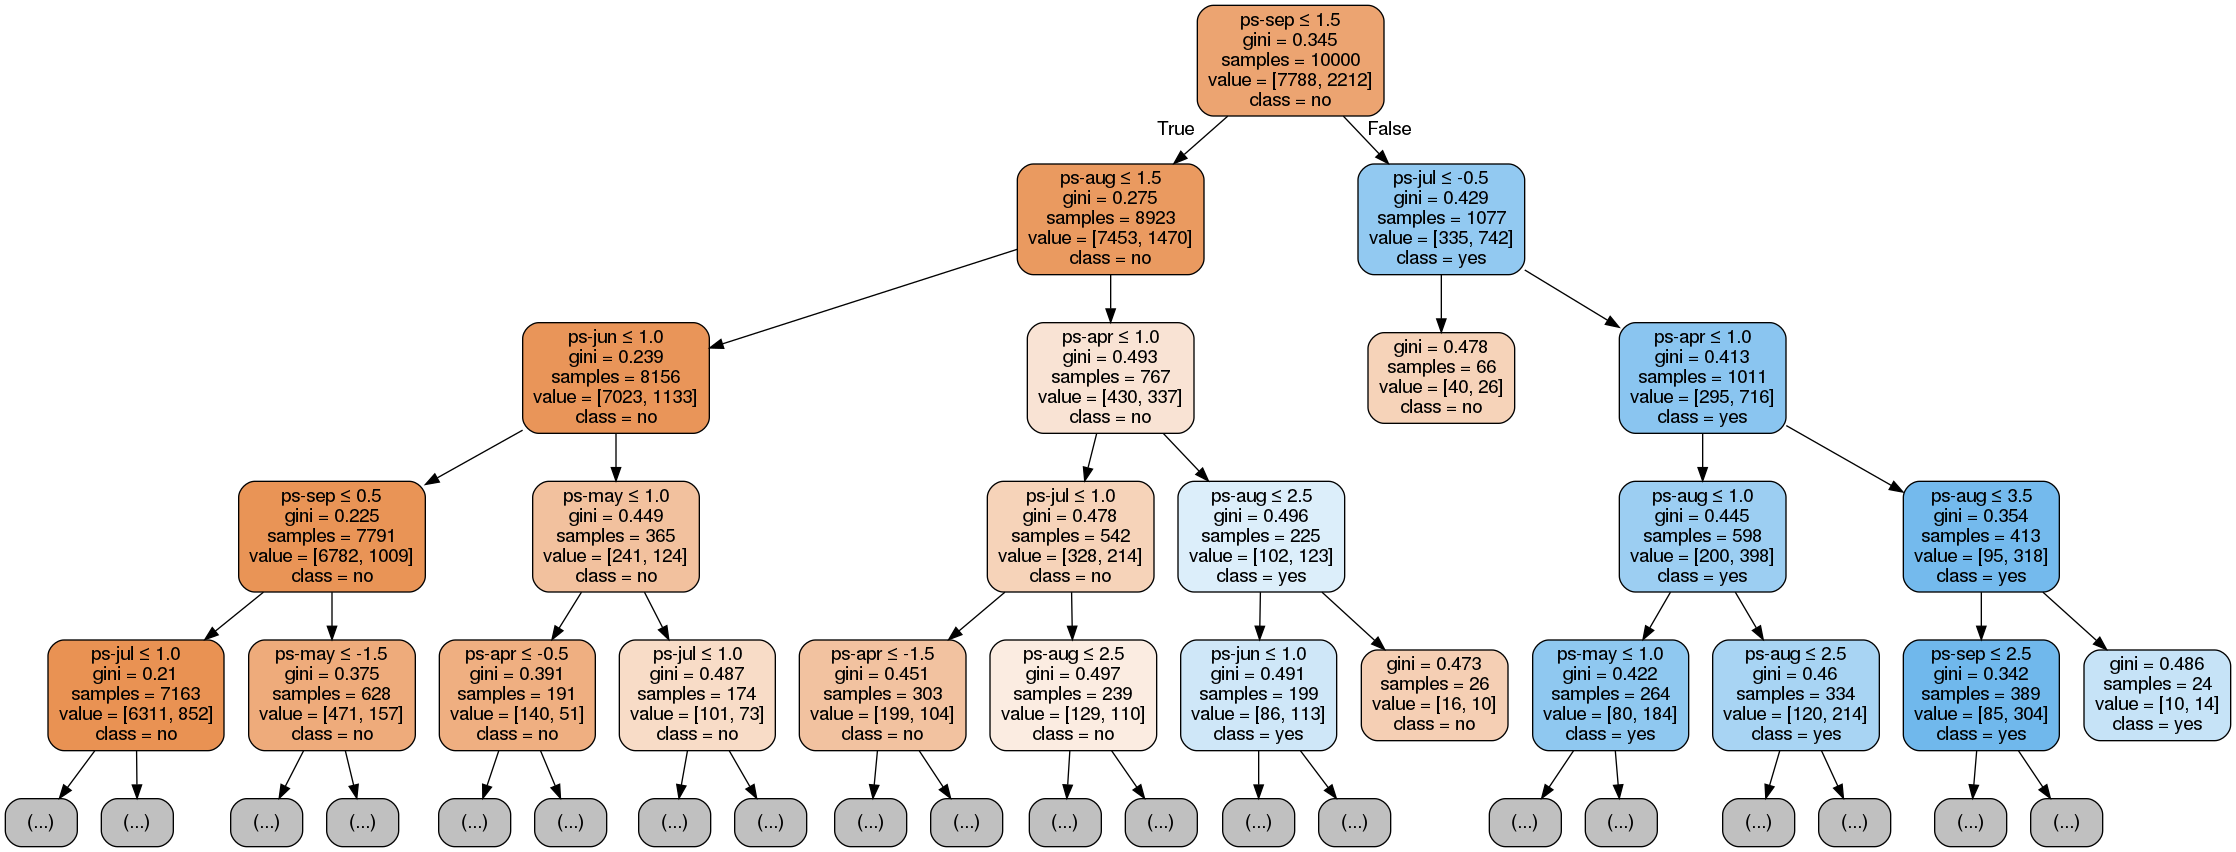
\includegraphics[width=\linewidth]{img/tree.png}
	\caption[LOF entry]{Primi quattro livelli dell'albero di decisione trovato}
	\label{tree}
\end{figure} 

I nostri tentativi sono continuati utilizzando altri due classificatori,
una \textit{neural network} e un \textit{KNN classifier}. Sul primo
abbiamo operato una grid search con i seguenti attributi e valori:

\begin{itemize}
	\item \texttt{activation} $\in [logistic, relu]$
	\item \texttt{alpha} $\in [1^{-5}, 1^{-6}, 1^{-7}]$
	\item \texttt{solver} $\in [lbfgs, sgd, adam]$
\end{itemize}

La rete neurale risultante era caratterizzata da $activation=relu$,
$alpha=1^{-7}$ e $solver=sgd$.

\begin{center}
	\begin{tabular}{c|c|c}
		\hline
		\textbf{Misure} & \textbf{Train} & \textbf{Test}\\
		\hline
		Accuracy & 0.82 & 0.81\\
		\hline
		Precision & 0.81 & 0.79\\
		\hline
		Recall & 0.82 & 0.81\\
		\hline
		F1 & 0.80 & 0.79\\
		\hline
	\end{tabular}
\end{center}

Infine, abbiamo tentato con \textit{KNN Classifier} che ha dato i risultati
pi\`u interessanti. In primo luogo, iterando con diversi valori di
\textit{n\_neighbors} abbiamo trovato il valore ideale a 150 e con pesi
uniformi.

\begin{center}
	\begin{tabular}{c|c|c}
		\hline
		\textbf{Misure} & \textbf{Train} & \textbf{Test}\\
		\hline
		Accuracy & 0.82 & 0.81\\
		\hline
		Precision & 0.81 & 0.79\\
		\hline
		Recall & 0.82 & 0.81\\
		\hline
		F1 & 0.80 & 0.79\\
		\hline
	\end{tabular}
\end{center}

In questo caso il classificatore non differisce molto dagli altri,
ma nel caso in cui si settino i pesi proporzionali alla distanza
(ovvero i vicini pi\`u prossimi influenzano maggiormente l'unit\`a
presa in esame) si registrano i valori pi\`u alti di recall e con
minima perdita di accuracy.

\begin{center}
	\begin{tabular}{c|c|c}
		\hline
		\textbf{Misure} & \textbf{Train} & \textbf{Test}\\
		\hline
		Accuracy & 0.82 & 0.81\\
		\hline
		Precision & 0.83 & 0.81\\
		\hline
		Recall & 0.84 & 0.83\\
		\hline
		F1 & 0.83 & 0.82\\
		\hline
	\end{tabular}
\end{center}

\section{Valutazione miglior modello}
Come descritto in precedenza, il nostro obiettivo era mettere in
risalto che la misura pi\`u importante da considerare
in questo caso, a nostro avviso, \`e la recall.
Per tanto il miglior classificatore trovato \`e stato il
\textit{KNN classifier} con numero di vicini uguale a 100
e con pesi proporzionali alla distanza dei vicini.
